\section{Main Window} 
If you run the GUI, the main window will be shown. It consists of a menu bar and several panels which cover a special topic respectively. Hint: If another window pops up labeled \emph{vagc}, this is the graphics card of the emulator.

\begin{figure}[H]
\begin{center}
	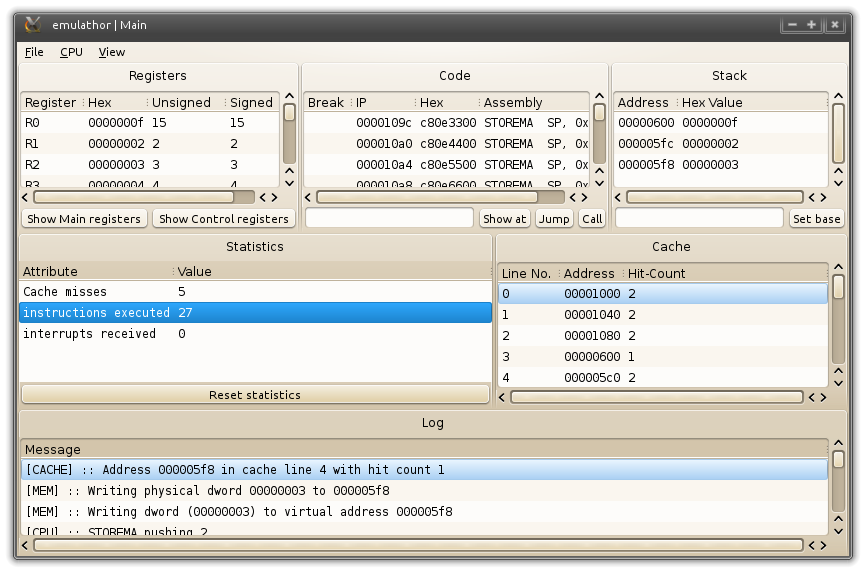
\includegraphics[width=0.8\textwidth]{./files/emu_gui_main.png}
\end{center}
	\caption{The main window of the GUI.}
\end{figure}

\subsection{Menu Bar}
\subsubsection{Loading a program}
You can load a program by clicking \emph{File} $\rightarrow$ \emph{Load image file}.

\begin{figure}[H]
\begin{center}
	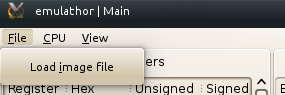
\includegraphics[width=0.5\textwidth]{./files/emu_gui_menu_file.png}
\end{center}
	\caption{The menu option to load a program.}
\end{figure}

A dialog appears where a file can be selected. Select a program which was previously assembled. The GUI can't detect if you chose a correct file because an assembled program is just a binary file where each four bytes are interpreted as an instruction. To find out if the program actually is a correct program just have a look at the code panel. If it doesn't recognise an instruction, it's probably a wrong or not compiled program.

\begin{figure}[H]
\begin{center}
	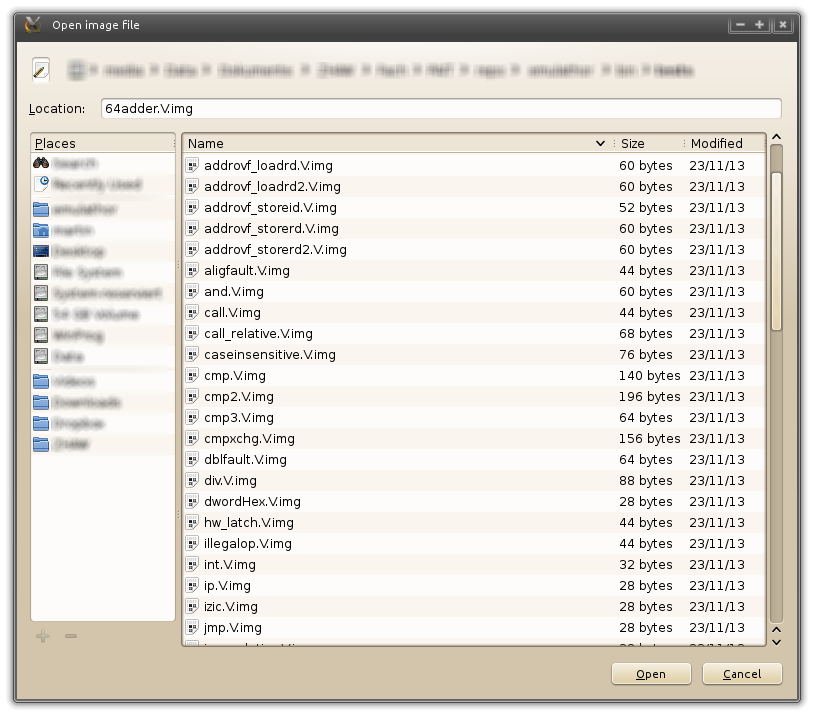
\includegraphics[width=0.8\textwidth]{./files/emu_gui_menu_filechooser.png}
\end{center}
	\caption{Choose an assembled program.}
\end{figure}

\subsubsection{Control the CPU}
With the menu options under \emph{CPU} you can control the CPU. The options control the CPU as follows:

\begin{description}
\item[Step] Executes one instruction then stops the execution
\item[Run] Executes the next instructions until a breakpoint or a \emph{STOP} instruction appears
\item[Stop] Stops the execution of a running program
\end{description}

\begin{figure}[H]
\begin{center}
	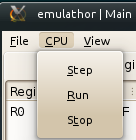
\includegraphics[width=0.2\textwidth]{./files/emu_gui_menu_cpu.png}
\end{center}
	\caption{The CPU menu.}
\end{figure}

\subsubsection{Open additional windows}
From the menu \emph{view} you can open additional windows.
\begin{description}
\item[Memory] Opens the memory inspection window
\item[Page Directory] Opens the page directory inspection window
\end{description}

\begin{figure}[H]
\begin{center}
	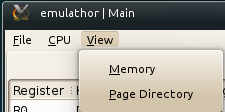
\includegraphics[width=0.3\textwidth]{./files/emu_gui_menu_view.png}
\end{center}
	\caption{Open additional windows.}
\end{figure}

\subsection{Panel Registers}
The registers panel allows you to monitor the registers of the emulator. The buttons below allow you to switch between the control and the main registers. Each register is displayed with its value. The value is printed as a hexadecimal, unsigned and signed value. 

\begin{figure}[H]
\begin{center}
	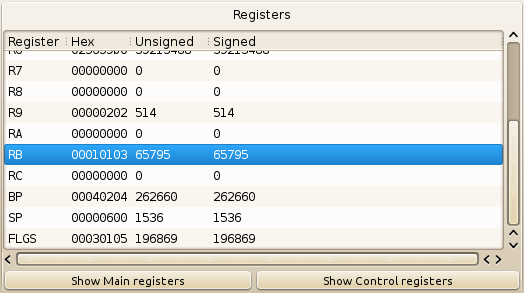
\includegraphics[width=0.8\textwidth]{./files/emu_gui_registers_main.png}
\end{center}
	\caption{Monitor the main registers of the emulator.}
\end{figure}

\begin{figure}[H]
\begin{center}
	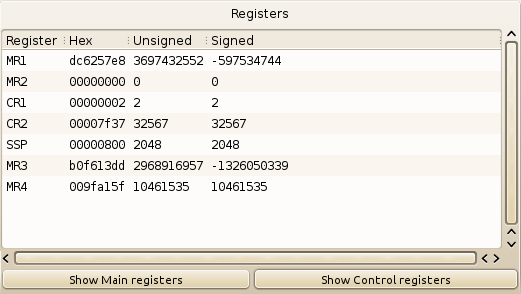
\includegraphics[width=0.8\textwidth]{./files/emu_gui_registers_control.png}
\end{center}
	\caption{Monitor the control registers of the emulator.}
\end{figure}

\subsection{Panel Code}
The code panel shows the disassembled code of the program. The columns have the following meaning:
\begin{description}
\item[Break] Indicates if a breakpoint is set at the corresponding address
\item[IP] Displays the address of the instruction in memory
\item[Hex] Displays the value of the instruction as hexadecimal number
\item[Assembly] Displays the disassembled instruction as text
\end{description}
The buttons below allow to control the program flow and what part of the program should be displayed. Enter an address in the input field an click one of the buttons.
\begin{description}
\item[Show at] Displays the part of the program from the entered address.
\item[Jump] Performs a \emph{JMP} instruction to the entered address.
\item[Call] Performs a \emph{CALL} instruction to the entered address.
\end{description}

\begin{figure}[H]
\begin{center}
	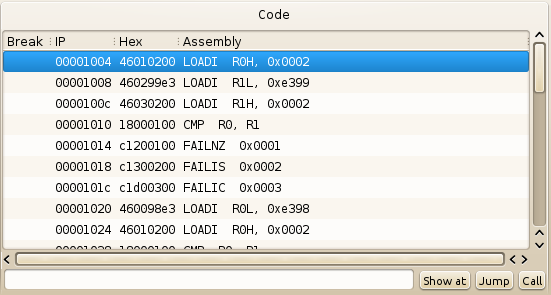
\includegraphics[width=0.8\textwidth]{./files/emu_gui_code_main.png}
\end{center}
	\caption{The code panel.}
\end{figure}

\subsubsection{Breakpoint}
A breakpoint can be set by double-clicking on the desired row, where the execution should be stopped.
\begin{figure}[H]
\begin{center}
	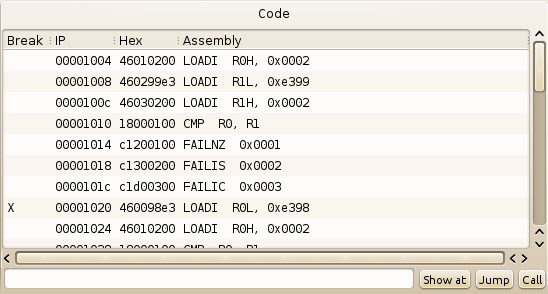
\includegraphics[width=0.8\textwidth]{./files/emu_gui_code_breakpoint.png}
\end{center}
	\caption{A breakpoint was set at the address 0x00001020.}
\end{figure}

\subsection{Panel Stack}
The stack panel allows you to monitor the stack. The stack can be anywhere in memory, therefore you can tell the GUI where the start of the stack is. The elements on the stack then are calculated with that base address and the current stack pointer.
\begin{figure}[H]
\begin{center}
	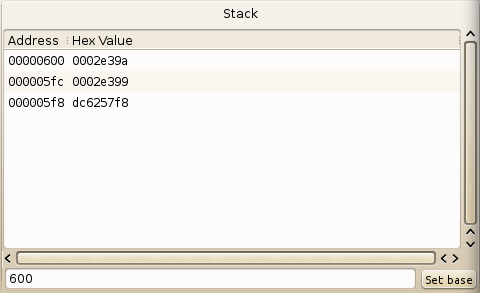
\includegraphics[width=0.8\textwidth]{./files/emu_gui_stack.png}
\end{center}
	\caption{The stack on address 0x00000600 with three items pushed.}
\end{figure}

\subsection{Panel Statistics}
The statistics panel shows some additional statistics. The statistics are only  reset by pressing the \emph{Reset statistics} button.
\begin{figure}[H]
\begin{center}
	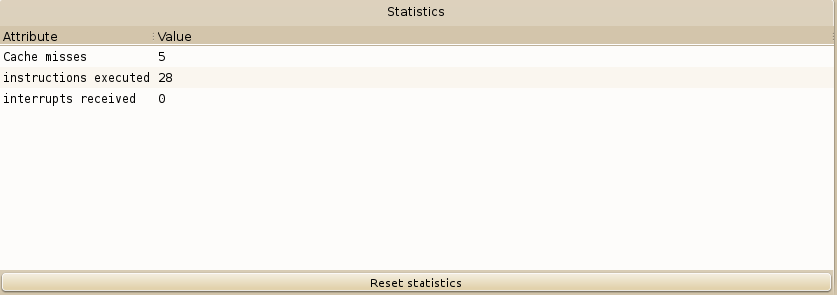
\includegraphics[width=0.8\textwidth]{./files/emu_gui_statistics.png}
\end{center}
	\caption{The statistics panel.}
\end{figure}

\subsection{Panel Cache}
The cache panel displays the cache lines. Each of the 16 lines has a number, a start address of the memory block being cached and a hit count.
\begin{figure}[H]
\begin{center}
	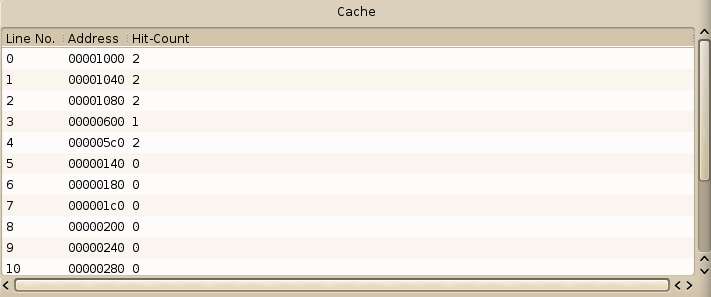
\includegraphics[width=0.8\textwidth]{./files/emu_gui_cache.png}
\end{center}
	\caption{The cache panel.}
\end{figure}

\subsection{Panel Log}
The log panel displays more detailed output of the emulator. It allows you to understand what the CPU did while executing the previous instruction. The log is cleared after executing an instruction.
\begin{figure}[H]
\begin{center}
	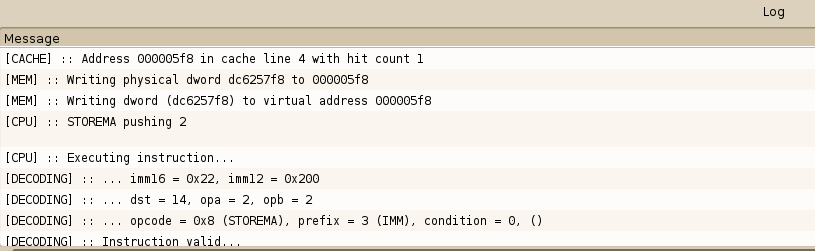
\includegraphics[width=0.8\textwidth]{./files/emu_gui_log.png}
\end{center}
	\caption{The log panel.}
\end{figure}